\subsection{Experiments and discussion}
To validate our approach, we carry out a comprehensive experimental evaluation study.  We study our proposed approach from three different perspectives: 

\begin{comment}
\begin{enumerate}
\item time-accuracy trade-off
\item stage-wise analysis
\item noise analysis
\end{enumerate}

We shall start by discussing the time-accuracy trade-off study. This allows us to investigate the end-to-end accuracy of pipeline while trading off computational time.  We also do stage-wise analysis where each stage is evaluated independently of other. This helps us understand which stage represents the potential bottleneck in terms of performance. Additionally, we also conduct noise analysis to understand the robustness of our approach to the noise.
\end{comment}

\begin{enumerate}
\item time-accuracy trade-off: to investigate the end-to-end accuracy of pipeline while trading off computational time
\item stage-wise analysis: to helps us understand which stage represents the potential bottleneck in terms of performance
\item noise analysis: to understand the robustness of our approach to the noise.
\end{enumerate}

\vspace{5pt}
\subsubsection{Time-accuracy trade-off experiment}
In the time-accuracy trade off experiment, we study the trade-off the trade off between data processing time and detection accuracy.
%\footnote{The term ``accuracy'' is loosely used in terms of performance. The study uses $f1$ score as the evaluation metric}. 
We vary the control parameters such as the threshold in stage 1, and observe the time it takes to process the data along with the accuracy of the complete pipeline. Figure \ref{fig:time-acc-tradeoff-ar-mog} depicts the time-accuracy trade off for varying activity ratios (AR). The trade off curve depicts the f1 score on the y-axis and the normalized processing time on the x-axis. F1 score and normalized processing time are defined as: 
$$ f1 = \frac{2 \times precision \times recall}{precision + recall}$$
$$\text{normalized time} = \frac{\text{total time to process video data}}{\text{length of video data}}$$
where $precision$ and $recall$ carry the standard meaning. In this study, we use the f1 score as the evaluation metric as opposed to standard accuracy because we have unbalanced dataset with respect to classes. The dataset has much more background data (-ve class) as compared to trespassing data (+ve class). Therefore, f1 score shall give a more realistic picture of the performance. 

It is clear by Figure \ref{fig:time-acc-tradeoff-ar-mog} that as the f1 score goes up, the normalized processing time also goes up, indicating the trade off. Notice that as the AR decreases (as indicated on the different lines in figure \ref{fig:time-acc-tradeoff-ar-mog}), the trade off curve shifts to the left. This is because in a less active environment i.e.,low AR, stage 1 is able to filter out more frames and thus less frames need to be processed by stage 2. Thus the curve shifts to the left indicating less overall processing time is consumed.   

For any curve in Figure \ref{fig:time-acc-tradeoff-ar-mog}, with a given AR fixed, the top right point corresponds to a small value of the stage 1 threshold ($\tau$). As $\tau$ is increased, we move towards the left; consuming less time at the cost of lower quality performance (f1 score). This is expected as stage 1 filters more and more frames with an increasing threshold ($\tau$) and thus a lesser number of frames are processed by stage 2.The synthetic dataset parameters used in this experiment are shown in Table \ref{table:fig1_data_params}. 

\begin{figure}
    \centering
    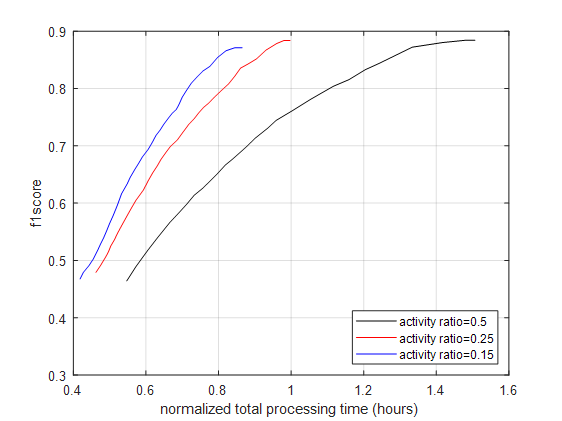
\includegraphics[width=\linewidth]{images/time-acc-tradeoff-ar-mog.png}
    \caption{Time-accuracy trade off for varying AR}
    \label{fig:time-acc-tradeoff-ar-mog}
\end{figure}

\begin{table}
\centering
\caption{Synthetic data parameters for time-accuracy trade off} \vspace{5pt}
\label{table:fig1_data_params}
\begin{tabular}{|l|l|}
\hline
parameter             & value  \\ \hline \hline
p                     & 1\%    \\ 
$\mu$    & 0.50\% \\ 
$\sigma$ & 0.20\% \\ \hline
\end{tabular}
\end{table}

\vspace{5pt}
\subsubsection{Stage-wise analysis study}
In this study, we independently analyse stage 1 and 2 using f1 score and Area Under the Curve (AUC). AUC has been used an additional metric since it measures the performance independent of any particular threshold and f1 score is useful in understanding the performance w-r-t threshold.  
%F1 score is primarily used for analysis as it helps in selecting optimum operating threshold. 
%Apart from that, we use AUC (Area Under the Curve) as the evaluation metric since it is not affected by class imbalance. We naturally have class imbalance since very few trespassing frames exist as compared to other frames. 
Table \ref{table:auc-time-analysis-s1} shows the AUC and mean processing time for each of the stages. Stage 1 has AUC of 0.94 whereas stage 2 shows an AUC of 0.81. The first stage takes 30 ms  (on average) to process a frame while stage 2 takes around 500 ms on $1080 \times 960$ sized frame. This shows that stage 1 is approx. $16.7$ times faster than stage 2 which resonates with our goal stated in Section \ref{sec:goal}. 

Figure \ref{fig:f1-analysis-mog} shows how the f1 score of stage 1 changes w-r-t threshold $\tau$ (percentage of foreground pixels). At $0.1\%$, it achieves a maximum f1 score of 0.91. Therefore, for our ARTS solution, we henceforth operate the stage 1 at this threshold.

\begin{figure}
    \centering
    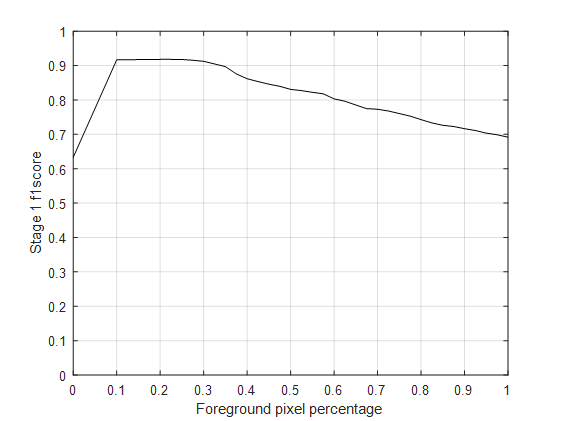
\includegraphics[width=\linewidth]{images/f1-analysis-mog.png}
    \caption{Stage 1 evaluation}
    \label{fig:f1-analysis-mog}
\end{figure}

Figure \ref{fig:f1-analysis-s2} shows the f1 score variation for stage 2. Y-axis indicates the f1 score whereas the x-axis varies prediction probability threshold $\nu$. We notice that maximum f1 score of 0.89 is achieved around $\nu=0.3$. Therefore, we opt to operate stage 2 at this threshold.

Note that Faster-RCNN, which is the backbone of our stage 2, produces multiple object predictions corresponding to each input image\footnote{image and frame have been used interchangeably in this text}. However, we model our stage 2 as a binary classification of the input frame as trespassing activity frame or other activity frame. Therefore, we map Faster-RCNN predictions to binary labels, i.e., trespassing or other. For the purpose of evaluation, we define a frame to exhibit trespassing activity if there is at least one valid person detection. A person detection is said to be valid if the probability of detection is above a particular threshold $\nu$, and the predicted bounding box sufficiently overlaps (i.e. $IOU >0.5$) with some ground truth bounding box. Mathematically speaking:
$$
\text{prediction} = 
\begin{cases}
% 1, &    \text{\footnotesize{if there is at least one valid person detection}} \\
1, &    \text{if any valid person detection exists} \\
0, &    \text{otherwise}
\end{cases}
$$
where \\
$\text{valid person detection} = \hat{p}_i>\nu \quad \& \quad IoU(\hat{b}_i,b_j)>0.5,$ \\
$\hat{b}_i =i^{th} \text{ prediction bounding box,}$ \\
$b_j =j^{th} \text{ ground truth bounding box,}$ \\
$\hat{p}_i = i^{th} \text{ prediction probability,}$ \\
$\nu =  \text{prediction probability threshold.}$

\begin{figure}
    \centering
    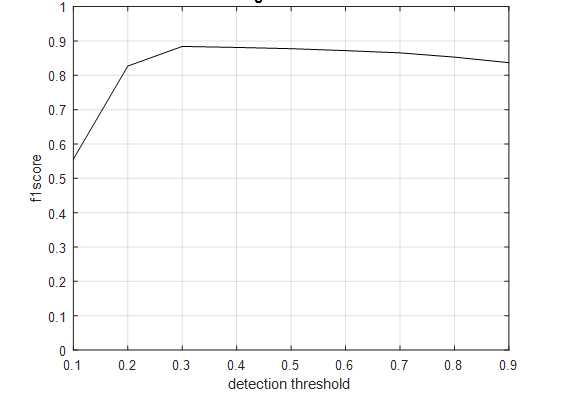
\includegraphics[width=\linewidth]{images/f1-analysis-s2.png}
    \caption{Stage 2 evaluation}
    \label{fig:f1-analysis-s2}
\end{figure}



\begin{table}
\centering
\caption{Stage 1 AUC and time analysis} \vspace{5pt}
\label{table:auc-time-analysis-s1}
\begin{tabular}{|l|l|c|}
\hline
stage   	& AUC     & mean processing \\
            &         &  time (ms)  \\ \hline \hline
stage 1     & 0.94    & 30    \\
stage 2     & 0.81    & 500  \\ \hline
\end{tabular}
\end{table}

\vspace{5pt}
\subsubsection{Noise analysis experiments}
Third and final study of our experimental evaluation concerns noise analysis. In this part, we evaluate the robustness of stage 1 against noise. We have 3 parameters: $p, \mu, \text{ and } \sigma$ to define the level of noise. A description of these parameters is given in Table \ref{table:noise-params}. To study the influence of one parameter, we vary it while keeping the others constant. 

Table \ref{table:noise-analysis-auc-mog} shows AUC for stage 1 when varying $p$ and $\mu$. We use the noise parameters ($AR=0.5$, $\mu=0.5\%$, $\sigma=0.2\%$) while varying $p$, and ($AR=0.5$, $p=2\%$, $\sigma=0.2\%$) while varying $\mu$. For both $p$ and $\mu$, it is clear that an increase in the noise level decreases the AUC of stage 1.  This result is also confirmed by f1 score plots of the stage 1 (Figure \ref{fig:noise-analysis-mog-p} and \ref{fig:noise-analysis-mog-mu}). Figures \ref{fig:noise-analysis-mog-p} and \ref{fig:noise-analysis-mog-mu} show the effect of changes in $p$ and $\mu$ respectively. Figure \ref{fig:noise-analysis-mog-p} shows that as $p$ increases, the overall f1 score curve shifts downward. This indicates the degradation of performance with an increase in $p$. A similar observation is also seen in Figure \ref{fig:noise-analysis-mog-mu} that shows the effect of change in $\mu$. However, the change is less prominent in this case.  


\begin{table}
\centering
\caption{Noise analysis - AUC for varying $p$ and $\mu$ \newline
$p$ sweep: $AR=0.5$, $\mu=0.5\%$, $\sigma=0.2\%$ \newline
$\mu$ sweep: $AR=0.5$, $p=2\%$, $\sigma=0.2\%$ \newline }

\label{table:noise-analysis-auc-mog}

\begin{tabular}{l r}

\begin{tabular}{|l|l|}
\hline
$p$         & AUC  \\ \hline \hline
2\%         & 0.93   \\
4\%         & 0.87    \\ 
6\%         & 0.83      \\ 
8\%         & 0.78       \\ \hline
\end{tabular}


\begin{tabular}{|l|l|}
\hline
$\mu$         & AUC  \\ \hline \hline
0.5\%         & 0.93   \\
0.7\%         & 0.92    \\ 
0.9\%         & 0.91      \\ 
1.1\%         & 0.88       \\ \hline
\end{tabular}

\end{tabular}

\end{table}

\begin{figure}[ht]
    \centering
    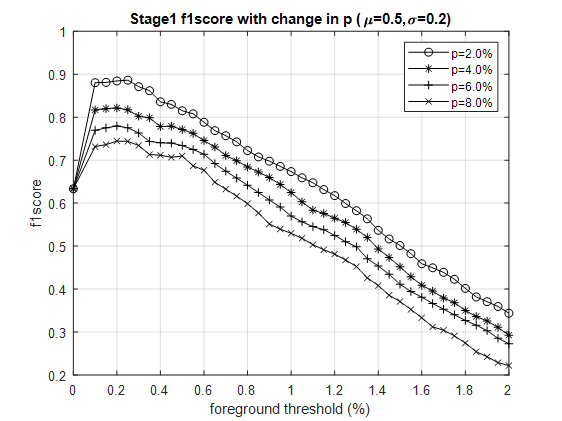
\includegraphics[width=\linewidth]{images/noise-analysis-mog-p.png}
    \caption{Noise analysis - varying $p$}
    \label{fig:noise-analysis-mog-p}
\end{figure}

\begin{figure}[ht]
    \centering
    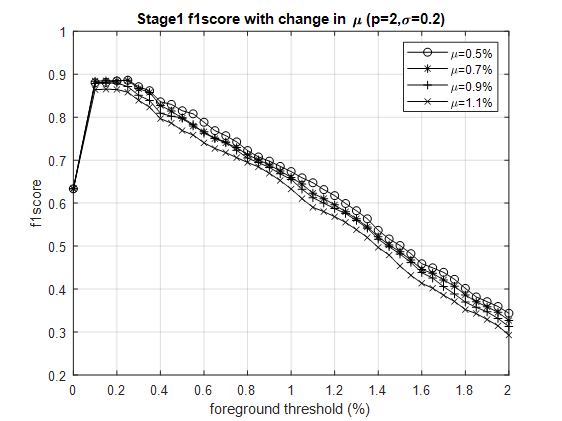
\includegraphics[width=\linewidth]{images/noise-analysis-mog-mu.png}
    \caption{Noise analysis - varying $\mu$}
    \label{fig:noise-analysis-mog-mu}
\end{figure}